%====================================================================================================
% FaultRecovery: A Ampliação da Biblioteca de Tolerância a Falhas
%====================================================================================================
% Apresentação do Trabalho de Conclusão de Curso
%----------------------------------------------------------------------------------------------------
% Autor				: Cleiton Gonçalves de Almeida
% Orientador		: Kleber Kruger
% Instituição 		: UFMS - Universidade Federal do Mato Grosso do Sul
% Campus    		: Coxim
%----------------------------------------------------------------------------------------------------
% Arquivo			: apresentacao.tex
% Data de criação	: 10 de Setembro de 2016
%----------------------------------------------------------------------------------------------------
% Beamer Presentation
% LaTeX Template
% Version 1.0 (10/11/12)
%----------------------------------------------------------------------------------------------------
% This template has been downloaded from:
% http://www.LaTeXTemplates.com
% License: CC BY-NC-SA 3.0 (http://creativecommons.org/licenses/by-nc-sa/3.0/)
%====================================================================================================

\documentclass[a4paper,12pt,brazil]{beamer}

\NeedsTeXFormat{LaTeX2e}[1995/12/01]

\RequirePackage[utf8]{inputenc}
\RequirePackage[portuguese,brazil]{babel}

\RequirePackage{amsmath,amssymb,amsfonts,float,fancyhdr}

%====================================================================================================
% Macro para dvi e pdf
%----------------------------------------------------------------------------------------------------
\usepackage{graphicx}
\usepackage{hyperref}
\usepackage{array}

\usepackage[font=small]{caption}
%\usepackage{caption}
\usepackage{subcaption}

%\hypersetup{colorlinks=true,citecolor=black,filecolor=black,linkcolor=black,urlcolor=black}
%\hypersetup[colorlinks=true,citecolor=blue,urlcolor=blue]{hyperref}

% caminho dos arquivos gráficos
\graphicspath{{figuras/}}
% extensões que não serão necessárias especificar em toda instancia de \includegraphics
\DeclareGraphicsExtensions{.pdf,.jpeg,.png}
%==================== Fim da macro para dvi e pdf ===================================================

%====================================================================================================
% Configurando formatação dos códigos-fontes
%----------------------------------------------------------------------------------------------------
\usepackage{listings}
\usepackage{color}
%\usepackage{courier}

% Altera o nome padrão do rótulo usado no comando \autoref{}
\renewcommand{\lstlistingname}{Quadro}

% Altera o rótulo a ser usando no elemento pré-textual "Lista de código"
\renewcommand{\lstlistlistingname}{Lista de Quadros}

% Configura a "Lista de Códigos" conforme as regras da ABNT (para abnTeX2)
\begingroup\makeatletter
\let\newcounter\@gobble\let\setcounter\@gobbletwo
\globaldefs\@ne \let\c@loldepth\@ne
%  \newlistof{listings}{lol}{\lstlistlistingname}
%  \newlistentry{lstlisting}{lol}{0}
\endgroup

% Cria uma nova customização para a linguagem C++
\lstset{
	alsoother={0123456789_},
	backgroundcolor=\color{white},
	basicstyle=\ttfamily,columns=fullflexible,
	breakatwhitespace=false,
	breaklines=true,
	captionpos=b,
	escapeinside={\%*}{*)},
	extendedchars=true,
	frame=shadowbox,
	inputencoding=utf8,
	keepspaces=true,
	numberbychapter=false,
	numbers=left,
%	numbersep=10pt,
	showspaces=false,
	showstringspaces=false,
	showtabs=false,
	tabsize=4,
	framextopmargin=5pt,
	framexbottommargin=5pt,
	framexleftmargin=5pt,
	framexrightmargin=5pt,
	language=C++,
	literate={á}{{\'a}}1 {ã}{{\~a}}1 {é}{{\'e}}1 {è}{{\`{e}}}1 {ê}{{\^{e}}}1 {ë}{{\¨{e}}}1 {É}{{\'{E}}}1 {Ê}{{\^{E}}}1 {û}{{\^{u}}}1 {ú}{{\'{u}}}1 {â}{{\^{a}}}1 {à}{{\`{a}}}1 {á}{{\'{a}}}1 {ã}{{\~{a}}}1 {Á}{{\'{A}}}1 {Â}{{\^{A}}}1 {Ã}{{\~{A}}}1 {ç}{{\c{c}}}1 {Ç}{{\c{C}}}1 {õ}{{\~{o}}}1 {ó}{{\'{o}}}1 {ô}{{\^{o}}}1 {Õ}{{\~{O}}}1 {Ó}{{\'{O}}}1 {Ô}{{\^{O}}}1 {î}{{\^{i}}}1 {Î}{{\^{I}}}1 {í}{{\'{i}}}1 {Í}{{\~{Í}}}1
}
%==================== Fim da configuração dos códigos-fontes ========================================

\mode<presentation>
{
	% The Beamer class comes with a number of default slide themes which change the colors and layouts of slides. Below this is a list % of all the themes, uncomment each in turn to see what they look like
	
	%\usetheme{default}
	%\usetheme{AnnArbor}
	%\usetheme{Antibes}
	%\usetheme{Bergen}
	%\usetheme{Berkeley}
	%\usetheme{Berlin}
	%\usetheme{Boadilla} % This is cool!
	%\usetheme{CambridgeUS}
	%\usetheme{Copenhagen}
	%\usetheme{Darmstadt}
	%\usetheme{Dresden} % This is cool!
	%\usetheme{Frankfurt}
	%\usetheme{Goettingen}
	%\usetheme{Hannover}
	%\usetheme{Ilmenau}
	%\usetheme{JuanLesPins}
	%\usetheme{Luebeck}
	\usetheme{Madrid} % This is cool!
	%\usetheme{Malmoe} % This is cool!
	%\usetheme{Marburg}
	%\usetheme{Montpellier}
	%\usetheme{PaloAlto}
	%\usetheme{Pittsburgh} % This is cool!
	%\usetheme{Rochester}
	%\usetheme{Singapore}
	%\usetheme{Szeged}
	%\usetheme{Warsaw}
	
	% As well as themes, the Beamer class has a number of color themes for any slide theme. Uncomment each of these in turn to see how it changes the colors of your current slide theme.
	
	%\usecolortheme{albatross}
	%\usecolortheme{beaver}
	%\usecolortheme{beetle}
	%\usecolortheme{crane}
	%\usecolortheme{dolphin}
	%\usecolortheme{dove} % (write, black)
	%\usecolortheme{fly}
	%\usecolortheme{lily} % (write, blue)
	%\usecolortheme{orchid}
	%\usecolortheme{rose}
	%\usecolortheme{seagull}
	%\usecolortheme{seahorse}
	%\usecolortheme{whale}
	%\usecolortheme{wolverine}
	
	%\setbeamertemplate{footline} % To remove the footer line in all slides uncomment this line
	%\setbeamertemplate{footline}[page number] % To replace the footer line in all slides with a simple slide count uncomment this line
	%\setbeamertemplate{navigation symbols}{} % To remove the navigation symbols from the bottom of all slides uncomment this line
}

%----------------------------------------------------------------------------------------------------
%	TITLE PAGE
%----------------------------------------------------------------------------------------------------

% The short title appears at the bottom of every slide, the full title is only on the title page
\title[Trabalho de Conclusão de Curso]{FaultRecovery: A ampliação da biblioteca de tolerância a falhas} 

\author{Cleiton Gonçalves de Almeida} % Your name
\institute[CPCX-UFMS] % Your institution as it will appear on the bottom of every slide, may be shorthand to save space
{
	Orientador: Prof. Me. Kleber Kruger \\ 
	Campus Coxim \\ 
	Universidade Federal de Mato Grosso do Sul \\ % Your institution for the title page 
	\medskip 
	\textit{cleitonufms@hotmail.com} % Your email address
}
\date{13 de Setembro de 2016} % Date, can be changed to a custom date

\begin{document}
	
	\begin{frame}
		\titlepage % Print the title page as the first slide
	\end{frame}
	
	\begin{frame}
		\frametitle{Estrutura da Apresentação} % Table of contents slide, comment this block out to remove it
		\tableofcontents % Throughout your presentation, if you choose to use \section{} and \subsection{} commands, these will automatically be printed on this slide as an overview of your presentation
	\end{frame}
	
	%------------------------------------------------------------------------------------------------
	%	PRESENTATION SLIDES
	%------------------------------------------------------------------------------------------------
	%====================================================================================================
% FaultRecovery: Ampliação da Biblioteca de Tolerância a Falhas
%====================================================================================================
% Apresentação do Trabalho de Conclusão de Curso
%----------------------------------------------------------------------------------------------------
% Autor				: Cleiton Gonçalves de Almeida
% Orientador		: Kleber Kruger
% Instituição 		: UFMS - Universidade Federal do Mato Grosso do Sul
% Campus     		: Coxim
%----------------------------------------------------------------------------------------------------
% Arquivo			: introducao.tex
% Data de criação	: 10 de setembro de 2016
%====================================================================================================

\section{Introdução} \label{Sec:Introducao}

\begin{frame}
	\frametitle{Introdução}
	\begin{itemize}
		\item Os sistemas embarcados (\textit{embedded computers} ou \textit{embedded systems}) correspondem a maior classe de computadores e abrangem uma grande faixa de aplicações e desempenhos;
		\item Com a expansão da computação ubíqua, os sistemas embarcados estão cada vez mais presentes no cotidiano das pessoas.
		\item É importante que esses sistemas tolerem falhas, pois defeitos nessas aplicações podem causar transtornos e prejuízos.		
		\end{itemize}
\end{frame}

\subsection{Justificativa}

\begin{frame}
	\frametitle{Justificativa}
	\begin{itemize}		
		\item Falhas podem ser causadas por:
		\begin{itemize}
			\item \textit{Bugs} de software;
			
			\item Questões ambientais;
			\begin{itemize}
				\item Interferências eletromagnéticas;
				\item Pulsos transitórios causados por prótons, íons pesadores e elétrons; Que podem causar um \textit{bit-flip}
			\end{itemize}			
			\item Problemas intrínsecos;
			\begin{itemize}
				\item Desgaste (envelhecimento) dos componentes de \textit{hardware};				
				\item Problemas de fabricação;
			\end{itemize}
		\end{itemize}
	\end{itemize}
\end{frame}

\subsection{Objetivos}

\begin{frame}
	\frametitle{Objetivo}
	\begin{itemize}
		\item Objetivo geral: Ampliar o injetor de falhas (FaultInjector ) e a biblioteca de recuperação de falhas (FaultRecovery) desenvolvidos por Kruger em sua dissertação
		de mestrado.
	\end{itemize}
\end{frame}

 % Introdução
	%====================================================================================================
% FaultRecovery: Ampliação da Biblioteca de Tolerância a Falhas
%====================================================================================================
% Apresentação do Trabalho de Conclusão de Curso
%----------------------------------------------------------------------------------------------------
% Autor				: Cleiton Gonçalves de Almeida
% Orientador		: Kleber Kruger
% Instituição 		: UFMS - Universidade Federal do Mato Grosso do Sul
% Campus     		: Coxim
%----------------------------------------------------------------------------------------------------
% Arquivo			: introducao.tex
% Data de criação	: 10 de setembro de 2016
%====================================================================================================

%\section{Revisão da Literatura} \label{Sec:Revisao}

%\subsection{Falhas, Erros e Defeitos}

%\begin{frame}
%	\frametitle{Falhas, erros e defeitos}
%	\begin{itemize}
%		\item As falhas estão associadas ao universo físico; os erros ao universo da informação; e os defeitos ao universo do usuário.
%		\item Uma falha não necessariamente leva a um estado de erro; e um erro não necessariamente provoca um defeito.
%	\end{itemize}
%\end{frame}
%
%\begin{frame}
%	\frametitle{Falhas, erros e defeitos}
%	\begin{figure}
%		\begin{center}\includegraphics[scale=0.5]{figuras/falhas_erros_defeitos}\end{center}
%		\caption[Universo dos erros]{Universo dos erros. Retirado de \cite{Weber:2003}.}
%		\label{Fig:FalhasErrosDefeitos}
%	\end{figure}
%\end{frame}

%\subsection{Classificação das Falhas}

%\begin{frame}
%	\frametitle{Classificação das falhas}
%	As falhas podem ser classificadas em:
%	\begin{itemize}
%		\item Duração
%		\begin{itemize}
%			\item Falhas transientes
%			\item Falhas intermitentes
%			\item Falhas permanentes
%		\end{itemize}
%		\item Extensão
%		\begin{itemize}
%			\item Falhas locais
%			\item Falhas globais
%		\end{itemize}
%		\item Natureza: hardware, software, projeto, entre outros.
%	\end{itemize}
%\end{frame}

\subsection{Tolerância a Falhas}

\begin{frame}
	\frametitle{Tolerância a falhas}
	\begin{itemize}
		\item Tolerância a falhas é a propriedade que permite a um sistema continuar funcionando adequadamente, mesmo que num nível reduzido, após a manifestação de falhas em alguns de seus componentes.
	\end{itemize}
\end{frame}

\subsection{Injeção de Falhas}

\begin{frame}
	\frametitle{Injeção de Falhas}
	\begin{itemize}
		\item A injeção de falhas é um processo importante para validar e verificar a confiabilidade de um sistema, seja por alteração de código, simulando uma falha de software ou a nível de pinos (Pin-level Injection) injetando falhas diretamente no hardware.
		\item Por que usar injetores de falhas ao invés de testar em um ambiente real?
	\end{itemize}
\end{frame}

\subsection{Padrão GoF (Padrões Fundamentais Originais)}

\begin{frame}
	\frametitle{Padrão de Projeto State}
	\begin{itemize}
		\item Padrões de comportamento são aqueles que descrevem como os objetos interagem, distribuindo responsabilidades.	
		\item O padrão State faz parte dos padrões de comportamento e permite que parte do comportamento de um objeto seja alterado conforme o estado do objeto.		
	\end{itemize}
\end{frame}

%\begin{frame}
%	\frametitle{Técnicas de Tolerância a Falhas: Exemplo de redundância}
%	\begin{figure}
%		\begin{center}\includegraphics[width=1.0\textwidth]{./figuras/nmr.png} \end{center}
%		\caption{Redundância de $n$ módulos. Retirado de \cite{Weber:2003}.}
%	\end{figure}
%\end{frame}

%\begin{frame}
%	\frametitle{Técnicas baseadas no temporizador \textit{watchdog}}
%	\begin{itemize}
%		\item O \textit{watchdog} é um dispositivo eletrônico temporizador usado para detectar erros e reiniciar o equipamento quando o sistema trava;
%		\item O mais comum são \textit{watchdogs} com dois registradores, um temporizador e outro, que armazena o valor de limiar. O temporizador deve ser zerado periodicamente pelo programa antes que atinja o valor do limiar.
%	\end{itemize}
%\end{frame}

%\begin{frame}
%	\frametitle{Técnicas de Tolerância a Falhas: Redundância de Software}
%	\begin{figure}
%		\begin{center}\includegraphics[width=1.0\textwidth]{./figuras/n_versoes.png} \end{center}
%		\caption{Programação $n$ versões. Retirado de \cite{Weber:2002}.}
%	\end{figure}
%\end{frame}

%\begin{frame}
%	\frametitle{Técnicas de Tolerância a Falhas: Redundância de Software}
%	\begin{figure}
%		\begin{center}\includegraphics[width=0.85\textwidth]{./figuras/blocos_recuperacao.png} \end{center}
%		\caption{Blocos de recuperação. Retirado de \cite{Weber:2002}.}
%	\end{figure}
%\end{frame}

%\begin{frame}
%	\frametitle{Técnicas de Tolerância a Falhas: Redundância de Dados}
%	\begin{itemize}
%		\item Consiste em ter dados redundantes na execução do programa.
%		\item Bits ou sinais extras são armazenados ou transmitidos junto a informação.
%		\item Tem sido utilizada exaustivamente em memórias e processadores através de códigos de correção de erros (CRC).
%	\end{itemize}
%\end{frame}

%\begin{frame}
%	\frametitle{Técnicas de Tolerância a Falhas: Redundância de Processamento}
%	\begin{itemize}
%		\item Repete a execução do código no tempo; 
%		\item Evita custos adicionais relativos ao hardware, mas aumenta o tempo necessário para realizar um processamento;
%		\item É usada em sistemas onde o tempo não é crítico ou onde o processador trabalha com ociosidade.
%	\end{itemize}
%\end{frame}

%\subsection{Injeção de Falhas}

%\begin{frame}
%	\frametitle{Injeção de falhas}
%	\begin{itemize}
%		\item A injeção de falhas é uma técnica de validação da segurança dos sistemas tolerantes a falhas que consiste na realização de experimentos controlados, nos quais observa-se o comportamento dos sistemas na presença de falhas geradas propositalmente (injetadas).
%		\item As injeções de falhas podem ser feitas via:
%		\begin{itemize}
%			\item Hardware
%			\item Software
%			\item Simulação
%		\end{itemize}
%		\item É necessário garantir a representatividade das falhas injetadas.
%		\begin{itemize}
%			\item O que injetar?
%			\item Onde injetar?
%		\end{itemize}
%	\end{itemize}
%\end{frame}

%\begin{frame}
%	\frametitle{Injeção de falhas por \textit{hardware}}
%	\begin{itemize}
%		\item As injeções podem ser classificadas em duas categorias:
%		\begin{itemize}
%			\item Sem contato (interferência eletromagnética, bombardeio com radiação ionizante, quedas de tensão na fonte de energia);
%			\item Com contato (\textit{pin-level}, que atua abrindo, curto-circuitando ou injetando sinais interferentes diretamente (por contato) em cada pino do dispositivo sob teste);
%		\end{itemize}
%		\item Requerem uso de \textit{hardware} especial;
%		\item Injetam falhas reais no \textit{hardware}, mas podem danificar o componente sob teste.
%	\end{itemize}
%\end{frame}

%\begin{frame}
%	\frametitle{Injeção de falhas por \textit{software}}
%	\begin{itemize}
%		\item SWIFI (\textit{Software Implemented Fault Injection}) - emula falhas de hardware através do software;
%		\item Menos dispendioso em termos de tempo e complexidade;
%		\item O sistema em estudo não corre o risco de ser danificado durante a injeção de falhas;
%		\item SFI (\textit{Software Fault Injection}). Um programa injetor emula as falhas no \textit{software} (\textit{bugs}) através da introdução de pequenas alterações no código original do programa;
%		\begin{itemize}
%			\item G-SWFIT (\textit{Generic Software Fault Injection Technique}).
%		\end{itemize}
%	\end{itemize}
%\end{frame}

%\begin{frame}
%	\frametitle{Trabalhos relacionados}
%	\begin{itemize}
%		\item A grande maioria são destinados a outras plataformas e a sistemas críticos ou de médio e grande porte;
%		\item Os trabalhos analisados não apresentavam as localizações das falhas injetadas;
%		\item O trabalho mais próximo foi o de Secall \cite{Secall:2007}.
%		\begin{itemize}
%			\item Fez uma avaliação comparativa do impacto do emprego das técnicas de programação defensiva na segurança de sistemas críticos.
%			\item Injetou falhas por interferências eletromagnéticas, utilizando-se radiofrequência irradiada.
%			\item Utilizou-se como estudo de caso um ambiente metroferroviário.
%			\item Ao final, foi feito uma avaliação quantitativa da eficácia de algumas técnicas de programação defensiva na capacidade de tolerância a falhas em aplicações críticas. 
%		\end{itemize}
%	\end{itemize}
%\end{frame}
 % Revisão da Literatura
	%====================================================================================================
% FaultRecovery: Ampliação da Biblioteca de Tolerância a Falhas
%====================================================================================================
% Apresentação do Trabalho de Conclusão de Curso
%----------------------------------------------------------------------------------------------------
% Autor				: Cleiton Gonçalves de Almeida
% Orientador		: Kleber Kruger
% Instituição 		: UFMS - Universidade Federal do Mato Grosso do Sul
% Campus     		: Coxim
%----------------------------------------------------------------------------------------------------
% Arquivo			: introducao.tex
% Data de criação	: 10 de setembro de 2016
%====================================================================================================

\section{Metodologia} \label{Sec:Metodologia}

\begin{frame}
	\frametitle{Metodologia}
	\begin{itemize}	
		\item Utilizou-se como ponto de partida as bibliotecas de injeção de falhas e de recuperação de falhas. 
		\item Para a ampliação das bibliotecas utilizou-se um microcontrolador \textit{mbed}, modelo NXP LPC1768. Este módulo é composto por:
		\begin{itemize}
			\item Núcleo ARM Cortex-M3 de 32 bits e 96 MHz de \textit{clock};
			\item Memória \textit{flash} com capacidade de 512 kB;
			\item Memória SRAM de 64 kB (32 kB SRAM destinados ao programa de usuário, e dois blocos adicionais SRAM de 16 kB para uso interno do microcontrolador);		
		\end{itemize}
	\end{itemize}
\end{frame}

\subsection{Injetor de Falhas}

\begin{frame}
	\frametitle{Biblioteca FaultInjector}	
		\begin{itemize}
			\item Na versão de Kruger a biblioteca FaultInjector permite simular o efeito do bit-flip em qualquer região de memória SRAM do microcontrolador mbed LPC1768, no entanto possuía duas limitações:
						
			\begin{itemize}
				\item Falta de flexibilidade, por não executar em outros modelos de microcontroladores.
				\item Impossibilidade de inserção de falhas na memória flash.
			\end{itemize}			
		\end{itemize}
\end{frame}

\begin{frame}
	\frametitle{Biblioteca FaultInjector}	
	\begin{itemize}
		\item Primeira limitação:
		\begin{itemize}			
			\item Foi possível criar uma única versão que automaticamente mapeia as
			regiões de memória dos modelos LPC1768, 66, 65 e 64.
		\end{itemize}
	\end{itemize}
\end{frame}

\begin{frame}
	\frametitle{Biblioteca FaultInjector}	
	\begin{itemize}
		\item Segunda limitação:
		\begin{itemize}			
			\item O interesse era explorar a memória flash ou seja, descobrir se seria possível injetar falhas nessa região de memória, uma vez que não era possível.
		\end{itemize}
	\end{itemize}	
	
\end{frame}

\subsection{FaultRecovery: Extensão da Biblioteca}

\begin{frame}
	\frametitle{Biblioteca FaultRecovery}	
	\begin{itemize}
		\item A biblioteca FaultRecovery foi criada para facilitar o uso de estratégias de tolerância e recuperação de falhas. Porém ela possuía algumas limitações:
		\begin{itemize}
			\item A estrutura da versão anterior não era baseada em um padrão de projeto.
			\item Utilizava funções por meio de defines (má prática).	
			\item Difícil modularização do código.	
		\end{itemize}
	\end{itemize}		
\end{frame}

\begin{frame}
	\frametitle{Biblioteca FaultRecovery}	
	\begin{itemize}
		\item Foi modificada para seguir o padrão \textit{State} forçando o usuário a implementar o \textit{firmware} como uma máquina de estados.
		\item Cada estado contém a sua classe de implementação, possibilitando a separação por responsabilidades.
		\item Possibilita a criação de pontos de recuperação de falhas.
	\end{itemize}		
\end{frame}

\begin{frame}
	\frametitle{Fluxograma da Biblioteca FaultRecovery}
	\begin{figure}
		\begin{center}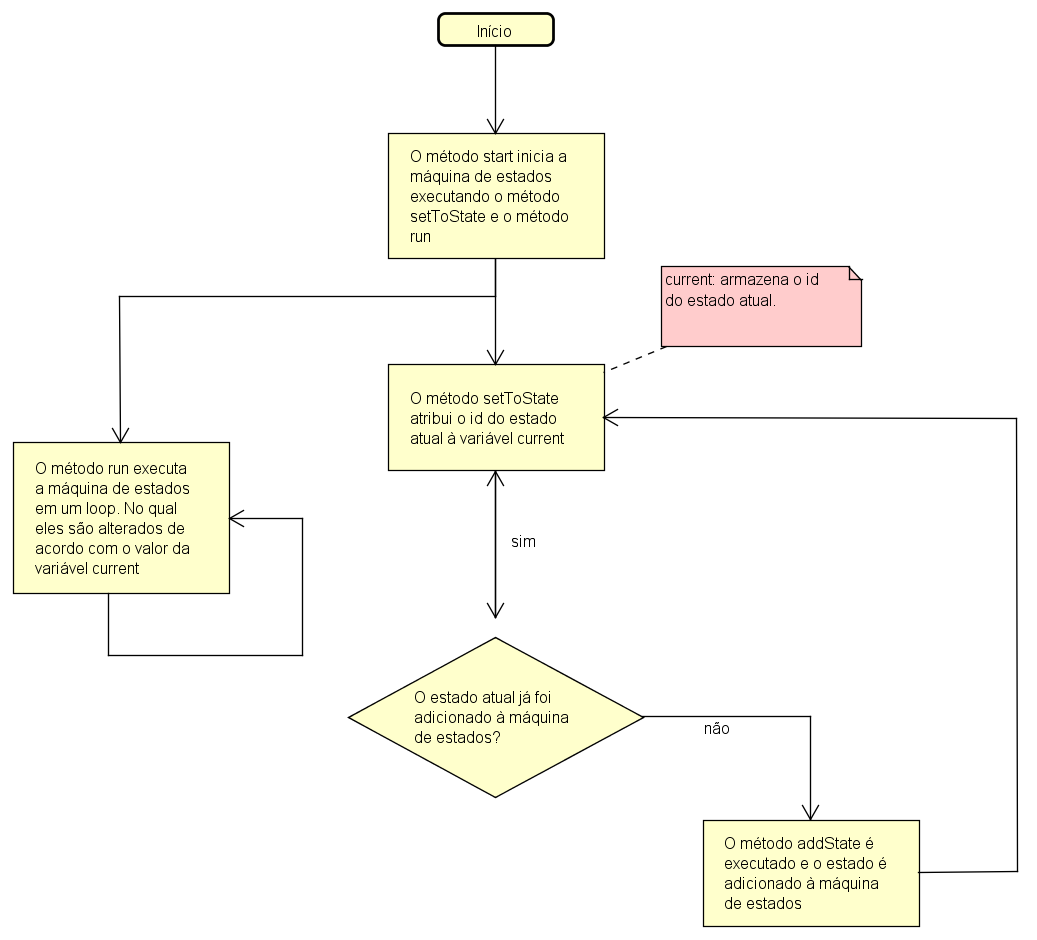
\includegraphics[width=0.6\textwidth]{figuras/fluxoFaultRecovery}\end{center}
		\caption{Fluxograma do funcionamento da máquina de estados da biblioteca.} \label{Fig:fluxoFaultRecovery}
	\end{figure}
\end{frame}

\subsection{Classe de Redundância de Dados: TData}

\begin{frame}
	\frametitle{Classe TData}	
		\begin{itemize}
			\item Redundância de dados automatizada tanto para variáveis primitivas quanto para objetos.
			\item O valor do objeto é armazenado em 3 cópias de segurança.
			\item As cópias são protegidas por um esquema de votação.
			\item Funciona com ponteiros e objetos de pilha.
			\item Mínima reescrita de código.
			\item Exemplo:
			\begin{itemize}
			\item TData$<$tipo\_da\_variável$>$ variavel(valor ou objeto).
			\end{itemize}		
		\end{itemize}		
\end{frame}


%\begin{frame}
%	\frametitle{Processo de leitura dos sensores}
%	\begin{figure}
%		\centering
%		\begin{subfigure}[t]{4.0in}
%			\centering
%			\includegraphics[scale=0.65]{figuras/le_sensores}
%			\caption{Sem injeção de falhas}\label{Fig:LeSensoresOrig}		
%		\end{subfigure}
%		\qquad
%		\begin{subfigure}[t]{4.0in}
%			\centering
%			\includegraphics[scale=0.65]{figuras/le_sensores_injeta_falhas}
%			\caption{Com injeção de falhas.}\label{Fig:InjecaoSensores}
%		\end{subfigure}
%		\caption{Processo de leitura dos sensores na estação meteorológica sem tolerância a falhas}\label{Fig:LeSensores}
%	\end{figure}
%\end{frame}

 % Metodologia
	%====================================================================================================
% FaultRecovery: Ampliação da Biblioteca de Tolerância a Falhas
%====================================================================================================
% Apresentação do Trabalho de Conclusão de Curso
%----------------------------------------------------------------------------------------------------
% Autor				: Cleiton Gonçalves de Almeida
% Orientador		: Kleber Kruger
% Instituição 		: UFMS - Universidade Federal do Mato Grosso do Sul
% Campus     		: Coxim
%----------------------------------------------------------------------------------------------------
% Arquivo			: introducao.tex
% Data de criação	: 10 de setembro de 2016
%====================================================================================================

\section{Resultados} \label{Sec:Resultados}

\begin{frame}
	\frametitle{Resultado do Desempenho da Biblioteca FaultRecovery}
	\begin{figure}
		\begin{center}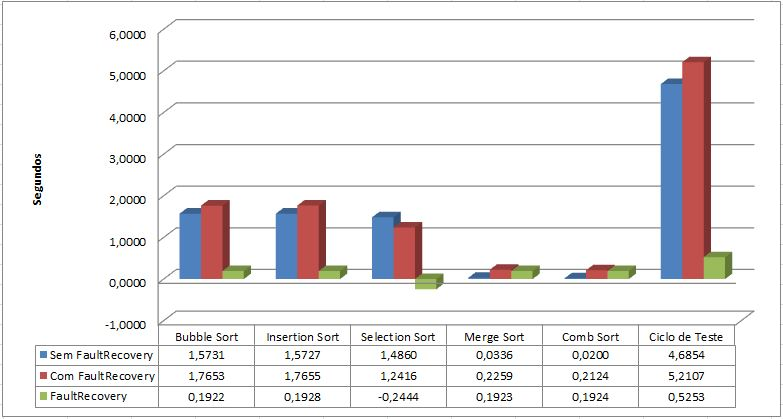
\includegraphics[width=0.92\textwidth]{./figuras/tempoRecovery.png}\end{center}
		\caption{Tempo de execução dos algoritmos de ordenação sem a biblioteca e com ela.}
	\end{figure}
\end{frame}

\begin{frame}
	\frametitle{Resultado do Desempenho da Biblioteca FaultRecovery}
	\begin{figure}
		\begin{center}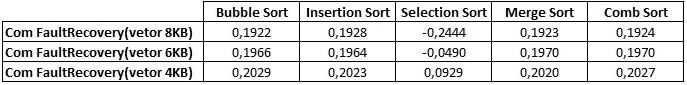
\includegraphics[width=1.0\textwidth]{./figuras/tempoRecovery2.png}\end{center}
		\caption{Tempo de execução da biblioteca FaultRecovery com três	vetores de tamanhos diferentes.}
	\end{figure}
\end{frame}

\begin{frame}
	\frametitle{Eficiência da Classe TData}
	\begin{figure}
		\begin{center}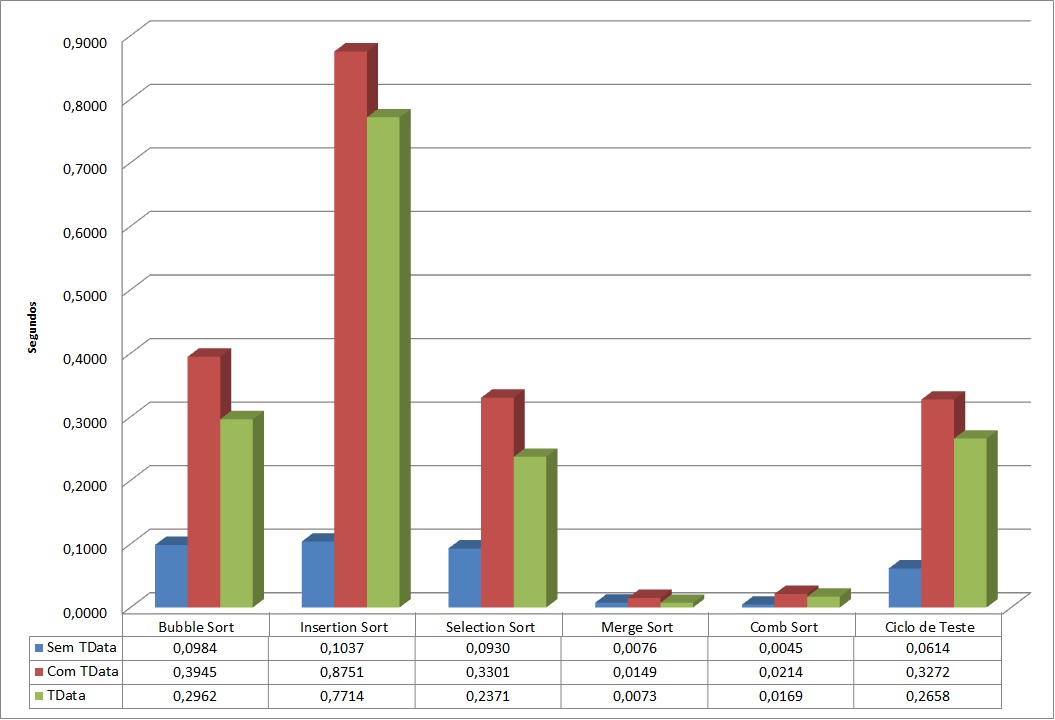
\includegraphics[width=0.8\textwidth]{./figuras/tempoTData.png}\end{center}
		\caption{O tempo de execução dos algoritmos sem a classe TData e com ela.}
	\end{figure}
\end{frame}

\begin{frame}
	\frametitle{Eficiência da Classe TData}
	\begin{figure}
		\begin{center}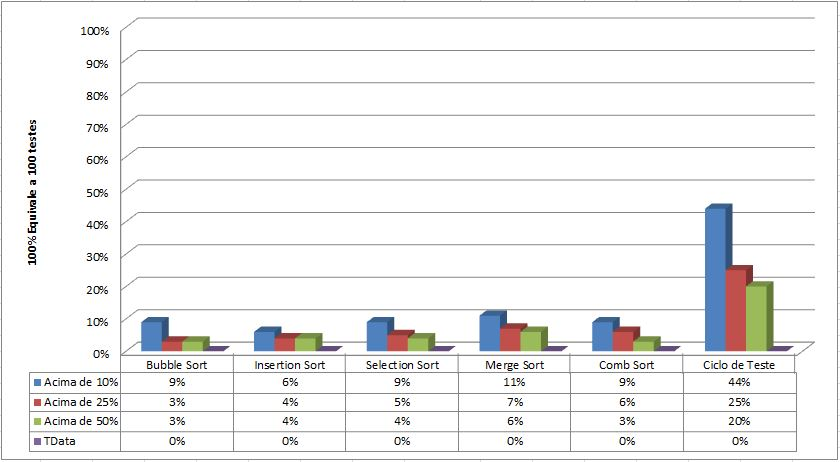
\includegraphics[width=1.0\textwidth]{./figuras/falhaTData.png}\end{center}
		\caption{Falhas detectadas nos teste.}
	\end{figure}
\end{frame}

\begin{frame}
	\frametitle{Recuperação de Falhas da Biblioteca FaultRecovery}
	\begin{figure}
		\begin{center}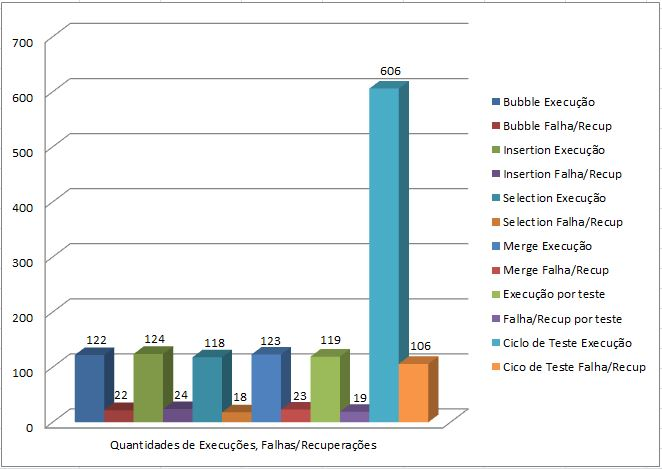
\includegraphics[width=0.82\textwidth]{./figuras/testeFaultRecovery.png}\end{center}
		\caption{Quantidade de execuções e falhas de cada algoritmo.}
	\end{figure}
\end{frame}

\begin{frame}
	\frametitle{Injeção de Falhas na Memória Flash}
	\begin{figure}
		\begin{center}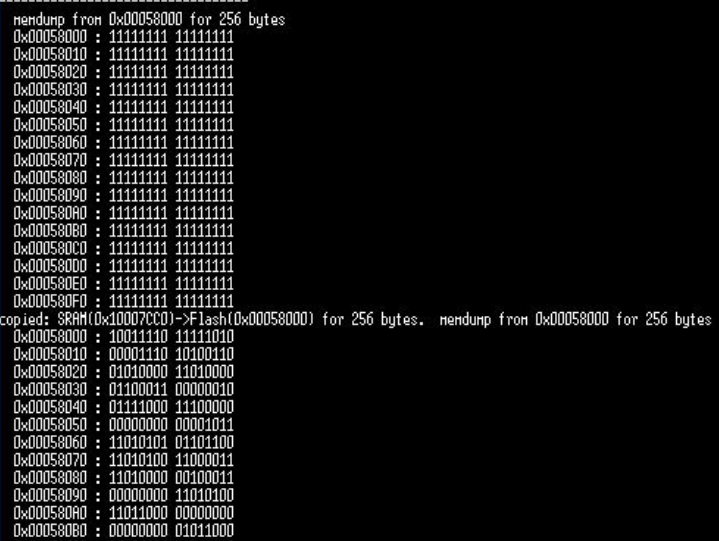
\includegraphics[width=0.72\textwidth]{./figuras/injecaoFlash.png}\end{center}
		\caption{Antes e depois dos bits serem modificados.}
	\end{figure}
\end{frame}
 % Resultados
	%====================================================================================================
% FaultRecovery: Ampliação da Biblioteca de Tolerância a Falhas
%====================================================================================================
% Apresentação do Trabalho de Conclusão de Curso
%----------------------------------------------------------------------------------------------------
% Autor				: Cleiton Gonçalves de Almeida
% Orientador		: Kleber Kruger
% Instituição 		: UFMS - Universidade Federal do Mato Grosso do Sul
% Campus     		: Coxim
%----------------------------------------------------------------------------------------------------
% Arquivo			: introducao.tex
% Data de criação	: 10 de setembro de 2016
%====================================================================================================

\section{Conclusão} \label{Sec:Conclusao}

\begin{frame}
	\frametitle{Conclusão}
	\begin{itemize}
		\item Sem a FaultRecovery:
		\begin{itemize}			
			\item O \textit{firmware} falhou e não continuou a sequência da máquina de estados.
		\end{itemize}
		\item Com a FaultRecovery:
		\begin{itemize}
			\item O \textit{firmware} falhou e continuou a sequência da máquina de estados de acordo com o ponto de recuperação configurado.	
			\item Aumento no tempo de execução do \textit{firmware}. No entanto a maioria das aplicações embarcadas não tem como fator principal o tempo de execução, exceto algumas aplicações de tempo real.
			
		\end{itemize}
	\end{itemize}
\end{frame}

\begin{frame}
	\frametitle{Conclusão}
	\begin{itemize}
		\item Sem redundância de dados:
		\begin{itemize}			
			\item Nenhuma falha foi tolerada.
			\item Num total de 100 testes, 44\% falharam.
		\end{itemize}
		\item Com redundância de dados:
		\begin{itemize}
			\item 100\% das falhas foram toleradas. No entanto adiciona um custo de desempenho no tempo de processamento. 
			\item Num total de 100 testes, nenhum teste falhou.
		\end{itemize}
	\end{itemize}
\end{frame}

\begin{frame}
	\frametitle{Contribuições deste trabalho}
	\begin{itemize}
		\item Parte da biblioteca FaultRecovery está sendo utilizada pelo Projeto de extensão Coxim robótica sediado na UFMS - campus Coxim para implementar uma máquina de estados para um carrinho seguidor de linha.
	\end{itemize}
\end{frame}

\begin{frame}
	\frametitle{Trabalhos Futuros}
	\begin{itemize}
		\item Testar o mapeamento de memória da biblioteca FaultInjector em outros modelos além do \textit{mbed} LPC1768.
		\item Salvar as cópias utilizadas pela classe TData, para se ter redundância de dados, em outras regiões de memória.
		\item Aperfeiçoar a biblioteca FaultRecovery e a classe TData para diminuir o tempo de processamento em uma aplicação embarcada.
		\item Explorar a injeção de falhas na memória flash, implementando um \textit{firmware} e injetando falhas enquanto ele está em execução.
	\end{itemize}
\end{frame}

\begin{frame}
	\frametitle{Trabalhos Futuros}
		\centering \resizebox{!}{2cm}{Obrigado!}
\end{frame}

 % Conclusão
	
	%------------------------------------------------------------------------------------------------
	%	REFERENCES SLIDES
	%------------------------------------------------------------------------------------------------	
	%====================================================================================================
% FaultRecovery: Ampliação da Biblioteca de Tolerância a Falhas
%====================================================================================================
% Apresentação do Trabalho de Conclusão de Curso
%----------------------------------------------------------------------------------------------------
% Autor				: Cleiton Gonçalves de Almeida
% Orientador		: Kleber Kruger
% Instituição 		: UFMS - Universidade Federal do Mato Grosso do Sul
% Campus     		: Coxim
%----------------------------------------------------------------------------------------------------
% Arquivo			: introducao.tex
% Data de criação	: 10 de setembro de 2016
%====================================================================================================

%\section{Referências Bibliográficas} \label{Sec:Referencias}

%\begin{frame}
%	\frametitle{Referências Bibliográficas}
%	\addcontentsline{toc}{chapter}{Referências Bibliográficas}
%	%\bibliographystyle{abnt}
%	\bibliographystyle{ieeetr} % Ordena por ordem de aparição.  
%	%\bibliographystyle{abbr} % Ordena por ordem alfabetica com nomes abreviados.
%	%\bibliographystyle{plain} % Ordena por ordem alfabetica com nomes por extenso.
%	\bibliography{bibliografia} % commented if *.bbl file included.
%\end{frame}

%\begin{frame}
%	\frametitle{Referências Bibliográficas}
%	\footnotesize
%	{
%		\begin{thebibliography}{99}	
%			\bibitem[Weber, 2003]{Weber:2003} Weber, T. S. (2003)
%			\newblock Tolerância a falhas: conceitos e exemplos.
%			\newblock \emph{Intech Brasil. Distrito 4 da ISA (The Instrumentation, System and Automation Society)}, 32 -- 42.
%		\end{thebibliography}
%	}
%\end{frame}
 % Referências Bibliográficas
	
\end{document}
